% !TEX TS-program = pdflatex
% !TEX encoding = UTF-8 Unicode

% This is a simple template for a LaTeX document using the "article" class.
% See "book", "report", "letter" for other types of document.

\documentclass[11pt]{article} % use larger type; default would be 10pt

\usepackage[utf8]{inputenc} % set input encoding (not needed with XeLaTeX)

%%% Examples of Article customizations
% These packages are optional, depending whether you want the features they provide.
% See the LaTeX Companion or other references for full information.

%%% PAGE DIMENSIONS
\usepackage{geometry} % to change the page dimensions
\geometry{a4paper} % or letterpaper (US) or a5paper or....
% \geometry{margin=2in} % for example, change the margins to 2 inches all round
% \geometry{landscape} % set up the page for landscape
%   read geometry.pdf for detailed page layout information

\usepackage{graphicx} % support the \includegraphics command and options

% \usepackage[parfill]{parskip} % Activate to begin paragraphs with an empty line rather than an indent

%%% PACKAGES
\usepackage{booktabs} % for much better looking tables
\usepackage{array} % for better arrays (eg matrices) in maths
\usepackage{paralist} % very flexible & customisable lists (eg. enumerate/itemize, etc.)
\usepackage{verbatim} % adds environment for commenting out blocks of text & for better verbatim
\usepackage{subfig} % make it possible to include more than one captioned figure/table in a single float
\usepackage{ulem}  % Strikeout with sout
\usepackage{tabularx}
\usepackage{color}
% These packages are all incorporated in the memoir class to one degree or another...

%%% HEADERS & FOOTERS
 \usepackage{lastpage}
 \usepackage{fancyhdr} % This should be set AFTER setting up the page geometry
 \pagestyle{fancy} % options: empty , plain , fancy
%\usepackage[automark]{scrpage2}
%\pagestyle{scrheadings}
\renewcommand{\headrulewidth}{1pt} % customise the layout...
\lhead{User Manual ITSecX}\chead{}\rhead{18.05.2015}
\lfoot{v 1.0.1}\cfoot{}\rfoot{\thepage of \pageref{LastPage}}

%%% SECTION TITLE APPEARANCE
\usepackage{sectsty}
\allsectionsfont{\sffamily\mdseries\upshape} % (See the fntguide.pdf for font help)
% (This matches ConTeXt defaults)

%%% ToC (table of contents) APPEARANCE
\usepackage[nottoc,notlof,notlot]{tocbibind} % Put the bibliography in the ToC
\usepackage[titles,subfigure]{tocloft} % Alter the style of the Table of Contents
\renewcommand{\cftsecfont}{\rmfamily\mdseries\upshape}
\renewcommand{\cftsecpagefont}{\rmfamily\mdseries\upshape} % No bold!

%%% END Article customizations

%%% The "real" document content comes below...

\title{Usermanual for ITSecX}
\author{Erik Brändli}
\date{21.05.2015} % Activate to display a given date or no date (if empty),
         % otherwise the current date is printed 

\begin{document}
\maketitle

\begin{tabular}{||l|l|l|l|l|}
	\hline
	\textbf{Version} & \textbf{Name} & \textbf{Datum} & \textbf{Status} & \textbf{Unterschrift} \\
	\hline
	\hline
	v 1.0.1us & Erik & \date{18.06.2015} & \color{red}{unstable} &  \\
\hline
	v 1.0.1ps & Erik & \date{18.06.2015} & \color{red}{pretty-stable} &  \\
\hline
	v 1.0.1s & Erik & \date{19.06.2015} & \color{red}{stable} &  \\
\hline
	v 1.0.1 & Hüseyin Bozkurt & \date{21.06.2015} & \color{green}{\textbf{Freigeben}} &  \\
	\hline
\end{tabular}

	


\pagebreak
\section{Inhaltsverzeichnis}
\tableofcontents


\pagebreak
\section{Einleitung}

EditierenITSecX ist die Abkürzung für "IT - Security - Extreme". ITSecX lässt sich mit dem von uns zur Verfügung gestellten Devices verbinden.\\
Die interne Syntax ist C \# . Das Hauptziel des Projektes ist es zu zeigen, wie einfach man Daten Abfangen und auswerten kann und Amateur Pen-Testern die Möglichkeit zu geben, schnell dynamisch an Ziele gelangen. Es ist auch möglich aus der zur Verfügung gestellten Software weit mehr rauszuholen (gegen Aufpreis).\\
Dieses Handbuch besteht vorranging aus einer Funktionsreferenz, Erläuterungen zu den wichtigsten Features und weitere ergänzende Informationen.

%Sie können dieses Handbuch in verschiedenen Formaten unter » http://www.php.net/download-docs.php herunterladen. Informationen dazu, wie dieses Handbuch erstellt wird, finden Sie %im Anhang unter dem Kapitel 'Über dieses Handbuch'. Wenn Sie sich für die Geschichte von PHP interessieren, lesen Sie bitte den entsprechenden Anhang.

\subsection{Autoren und Mitwirkende}

Das Projektteam bestand aus 5 Mitgliedern von denen aktuell noch 2 vorhanden sind. 

-) Erik Brändli 

-) Hüseyin Bozkurt

\sout{-) Markus Schulmeister}

\sout{-) Arian Sayah} 

\sout{-) Raied El'beidak}
\\ \\
Projektabnehmer:

-) Michael Borko

-) Werner Kristufek

-) Erich Trenner

-) Elisabeth Wildling

\subsection{Autoren und Editoren}

Folgende Personen verdienenen Anerkennung dafür, dass Sie wesentlichen Inhalt zum Handbuch beigetragen haben und/oder weiterhin beitragen werden: Hüsyein Bozkurt und Erik Brändli.

Vielen Dank!\\

\subsection{Einsatzgebiet}

Als Einsatzgebiet sind Schulen mit IT-Ausbildung gedacht, da man dort den Schülern lehren, kann wie einfach es ist ein Netzwerk auszutricksen bzw. um zu veranschaulichen, dass Netzwerksicherheit ein wichtiger Part in unserer Welt ist.

Denn die meisten Schüler denken, dass ihre Daten sicher sind, und dass niemand mitlesen kann!

\section{Vorbereitung des Produktes}
Sollten Sie bereits unser modifiziertes "Arch Linux" besitzen können Sie dieses Kapitel überspringen.
\subsection{Vorausgesetztes}
Um das Produkt zu verwenden erwerben Sie am besten unser "Arch Linux" von unserer Seite, oder Sie insatllieren sich zu Ihrer Arch Linux version folgende Pakete dazu:

-) Openssh

-) openbsd-netcat

-) nmap

-) tcpdump

-) dsiff

\subsection{Erstellen eines tcpdump-services}
Falls Sie nicht unser modifiziertes "Arch Linux" verwenden müssen Sie sich einen Service schreiben welches einen tcpdump startet auf einem von Ihnen ausgewählten Interface startet. Dieser Dump muss in eine Datei geschrieben werden, wie dies funktioniert finden sie auf der Seite von tcpdump.(http://www.tcpdump.org/)\\

\subsection{Erweiterungen}

Um folgende Dinge müssen Sie sich kümmern:

-) Es sollte sich der Tcpdump bei Systemstart von alleine starten.

-) Sudo befehl muss ohne Passwort erfolgen

\section{Installation des Produktes}

Führen Sie den gelieferten Installer aus um die Software zu installlieren.\\
AxNetworks ist eine wichtige externe Komponente, damit die Software auf dem Windowsgerät läuft.
Nach erfolgreicher Installation ist das Produkt voll einsatzbereit.\\

\section{Inbetriebnahme}

\pagebreak
\section{Funktionen}
In diesem Kapitel werden die Funktionen der Gui erklärt bezüglich ihrer Anwendung und Auswirkung \\
\subsection{Datei}
\subsubsection{IP Settings}
In "\textbf{IP Settings}" lässt sich festlegen zu welchem Device man sich verbinden möchte.\\
Man findet zwei maskierte Eingabefelder wieder. Das Eingabefeld mit IP-Address nimmt die IP-Adresse(v4) vom Device entgegen und validiert ob diese IP korrekt ist. Das Feld nimmt eine bis zu 4 stellige Zahl zur Definierung des Kommunikationis-Port am Device.\\
Mit dem Knopf "\textbf{Apply Settings}" können Sie die Einstellungen übernehmen. "Discard Settings" verwirft die temporäre Konfiguration.\\
%\color{green}{\textbf{Bild}}\color{black}
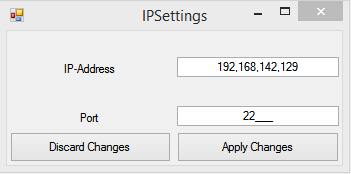
\includegraphics{IP_SETTINGS}
\subsubsection{Import $\rightarrow$ Settings}
\label{sec:FFIS}
Ermöglicht das Importieren von Konfigurationen bezüglich: 

-) \textbf{Verbindung-Punkt (IP:Port)}

-) \textbf{Authentifizierung (Username, Passwort)}\\
Ein OpenFile Dialog öffnet sich und bittet Sie darum eine Datei auszuwählen, eine \textbf{.conf} Datei (Die Sie mit unserer Software erstellten, siehe auch Kapitel \ref{sec:FFES})
Desweitern wird die Verbindung sofort getestet um zu überprüfen ob die übergebenen Daten korrekt sind, und das Device verfügbar ist.
\textbf{Dies kann in gewissen Fällen länger dauern}.\\
\subsubsection{Export $\rightarrow$ Settings}
\label{sec:FFES}
Ermöglicht das Exportieren von Konfigurationen bezüglich: 

-) \textbf{Verbindung-Punkt (IP:Port)}

-) \textbf{Authentifizierung (Username, Passwort)}

-) Interface-Settings (Schriftfarbe, Hintergrundfarbe, \dots )\\
Desweitern wird empfohlen eine Setting erst dann zu exportieren wenn die Verbindung bereits getestet wurde.
\textbf{Diese Datei enthält sensible Daten bitte schützen Sie sich selbst, indem Sie diese Datei schützen}\\
\subsubsection{Verbindung $\rightarrow$ verbinden}
Über diesen Menupunkt verbindet man sich zum Device, dafür ist jedoch erforderlich, dass Sie Ihre Daten in die Felder "Username" \& "Passwort" eintragen.\
Danach bestätigen Sie Ihre Eingabe mit dem Button "\textbf{Apply + Login}", durch das klicken auf den Button probiert das Programm sich zu dem Device zu verbinden.\\
%\color{green}{\textbf{Bild}}\color{black}
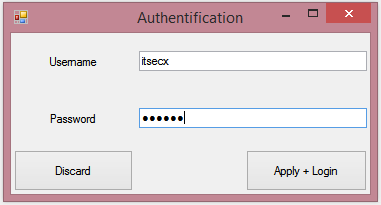
\includegraphics{VERBINDEN}
\subsubsection{Verbindung $\rightarrow$ trennen}
Mit der Funktion trennen lässt sich die Kommunizierschnittstelle zurücksetzen, folglich sind Sie vom Device getrennt. um sich erneut zu verbinden müssen Sie alle Settings neu eingeben, oder Sie laden eine Konfiguration über Import $\rightarrow$ Settings (\ref{sec:FFIS}) \\
\pagebreak
\subsection{Tools}
Hier befinden sich jene Tools die das Device ausführen kann, Konfigurationen für diese Tools werden automatisch geladen bzw. in einem Fenster für Sie bereit gestellt, dass sie nur mehr auswählen müssen wer \& was.\\
\subsubsection{Scanner $\rightarrow$ nmap}
nmap ("Network Mapper") ist ein Tool womit Sie einen fremden Computer:

-) prüfen können ob dieser Ein-/Aus-geschalten ist

-) schauen weleche Ports offen hat

-) evtl. erkennen welches Betriebsystem auf diesem Computer läuft.

-) wie weit dieser Computer entfernt ist
Hier bei ist nicht die Rede von wie viele Meter ist dieser Computer weg, sondern wieviele netzwerktechnische zwischen Punkte es gibt.\\
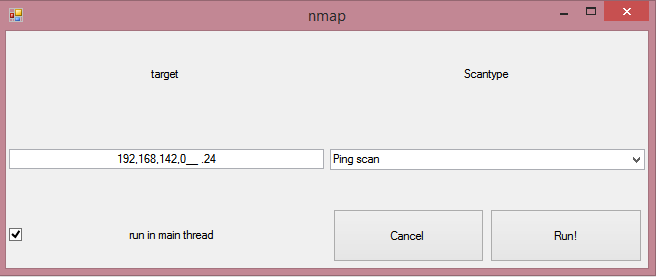
\includegraphics[width=0.8\textwidth]{nmap}
% \color{green}{\textbf{Bild}}\color{black}
\subsubsection{Sniffing $\rightarrow$ tcpdump $\rightarrow$ start/stop}
tcpdump legt die Netwerkpakete in einem Logfile(\textbf{.pcap}) ab. \\
Mit der Funktion \textbf{start} wird der "Dump" in eine Datei geschrieben.

\textbf{!} Sollte es bereits gestartet sein, wird dieser neugestartet.\\
Mit der Funktion \textbf{stop} wird der "Dump" angehalten. \\
%\color{green}{\textbf{Bild}}\color{black}
\pagebreak
\subsubsection{Direct Command}
Über diese Funktion ist es möglich einen Befehl am Device auszuführen, denn evtl. möchten Sie selbst etwas auslesen oder umstellen.\\
%\color{green}{\textbf{Bild}}\color{black}
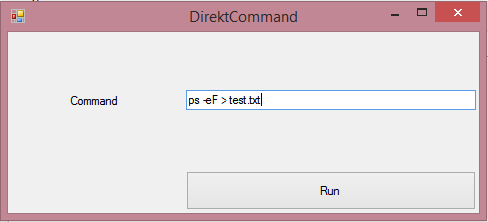
\includegraphics[width=0.8\textwidth]{direct_cmd}
\pagebreak
\subsection{Files}
Mit den Funktionen in diesem Menü können Sie mit den Logs und Datein arbeiten, also diese Anzeigen und herunterladen.\\
\subsubsection{View File}
Hier können Sie in dem Sie die auf der linken seite eine Datei auswählen diese anzeigen.\\
%\color{green}{\textbf{Bild}}\color{black}
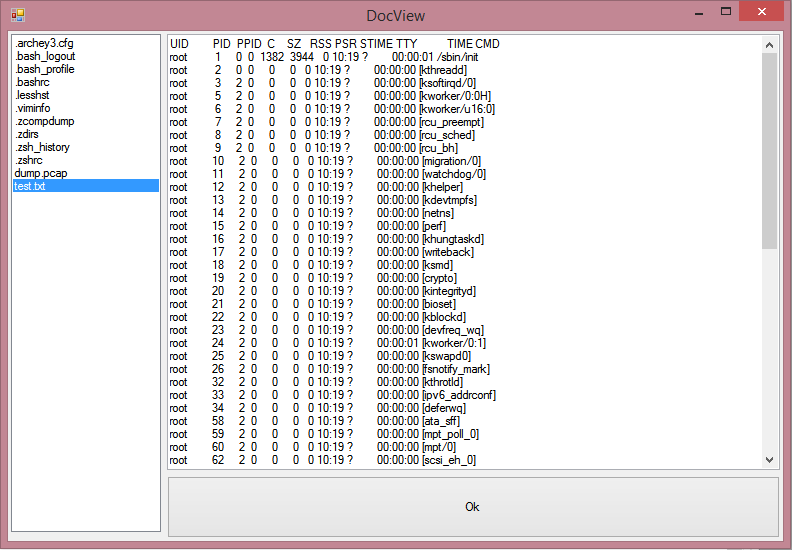
\includegraphics[width=0.8\textwidth]{view_file}
\pagebreak
\subsubsection{View tcpdump}
Wenn Sie diese Aktion ausführen wird der aktuelle tcpdump im Hauptfenster ausgegeben.\
\textbf{Da diese Daten erst konvertiert werden müssen kann dies eine gewisse Zeit in anspruch nehmen!}\\
%\color{green}{\textbf{Bild}}\color{black}
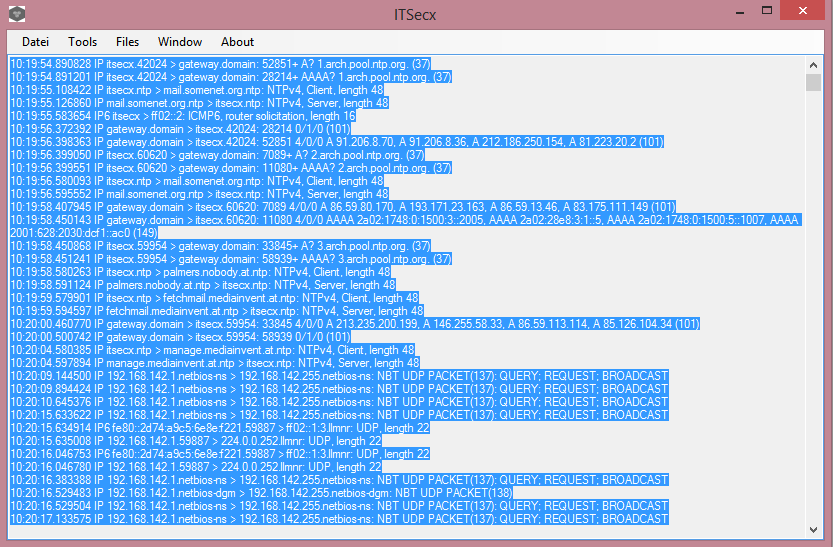
\includegraphics[width=0.8\textwidth]{view_tcpd}
\\
\subsubsection{View tcpdump $\rightarrow$ Download}
Sollten Sie diese Funktion auswählen kommt ein "speichern unter" Dialog diesen müssen Sie bestätigen, dann wird der aktuelle tcpdump an dieser Stelle gespeichtert.
\\
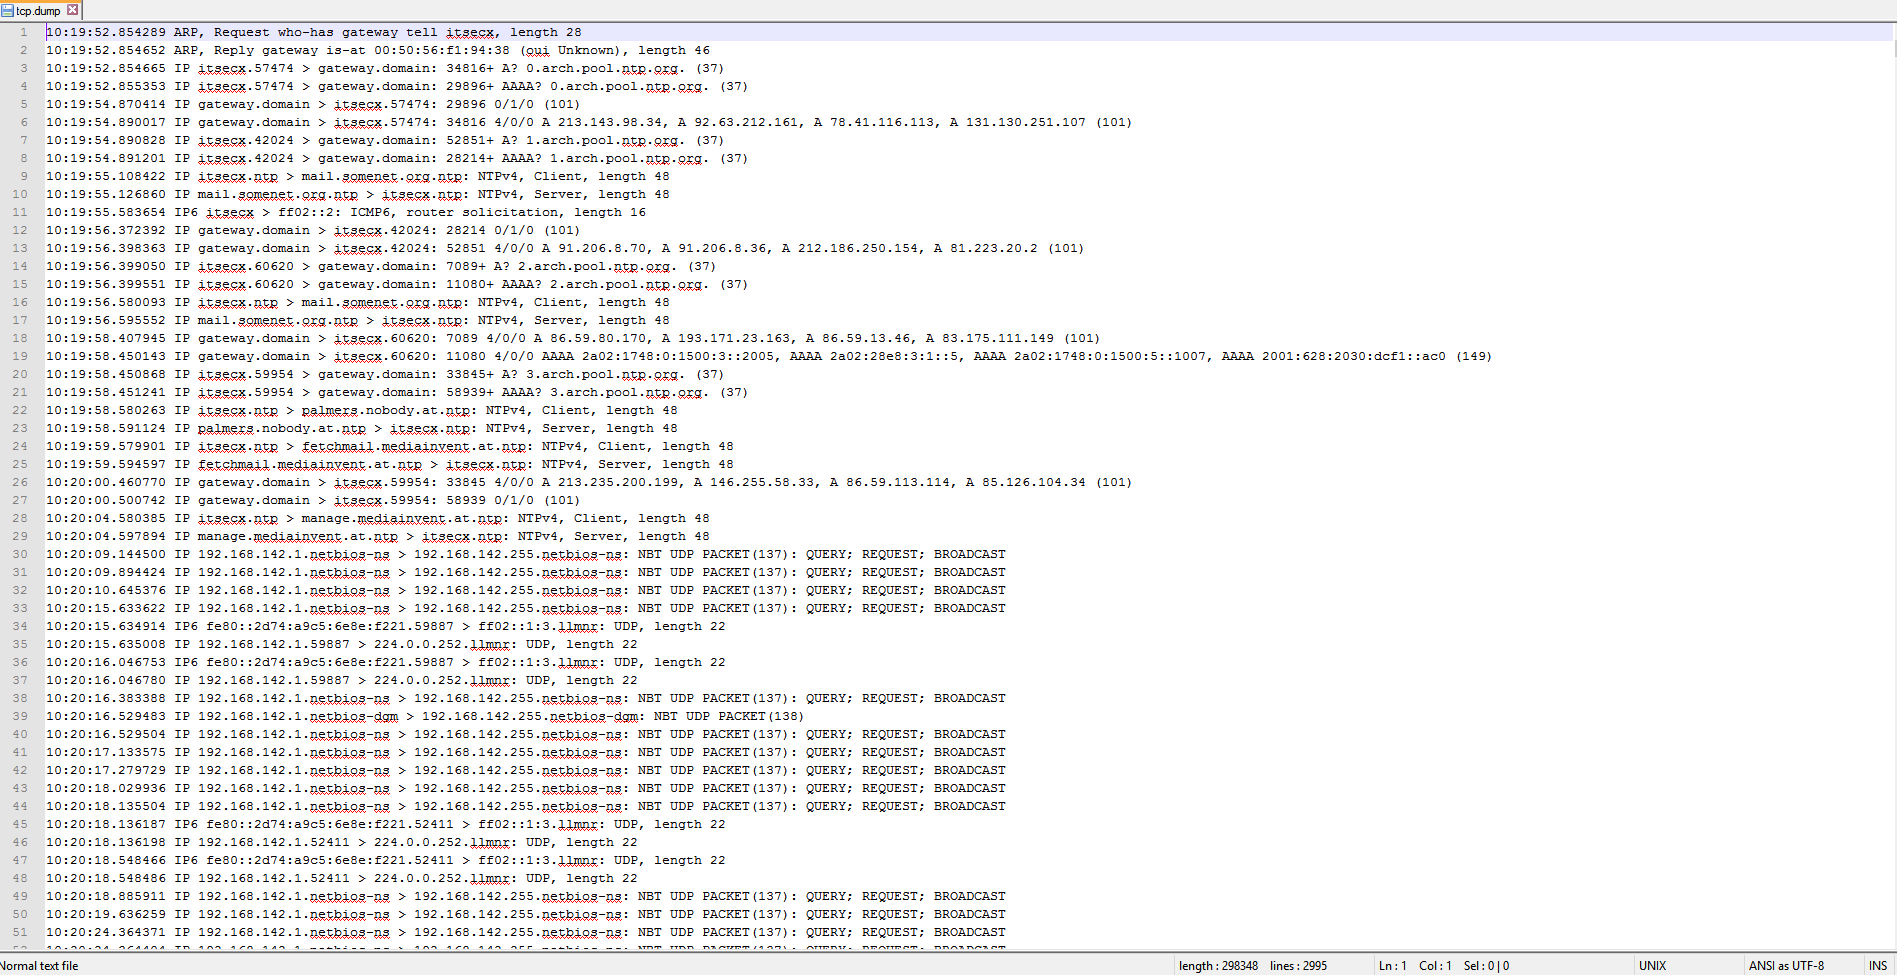
\includegraphics[width=0.8\textwidth]{tcpd}
%\color{green}{\textbf{Bild}}\color{black}
\\
\pagebreak
\subsection{Window}
In diesem Menüpunkt können Sie den angezeigten Ausgabetext optisch bearbeiten.\\
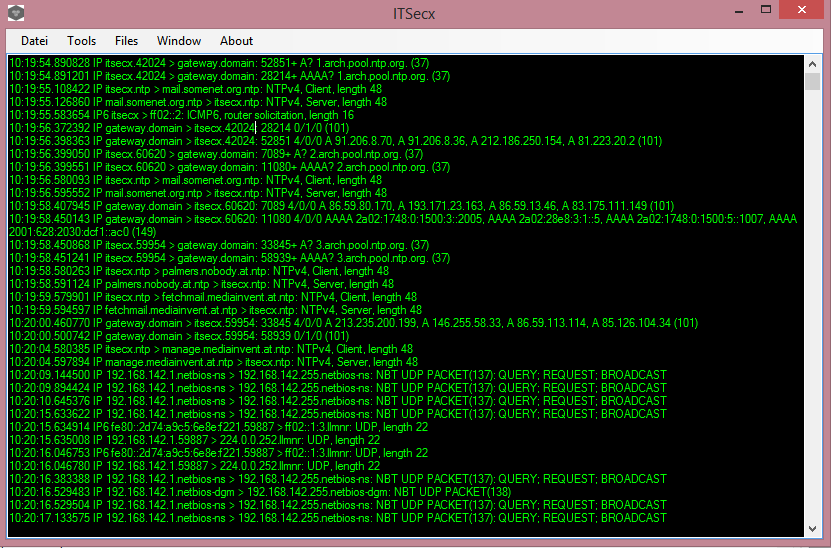
\includegraphics[width=0.8\textwidth]{colors}
%\color{green}{\textbf{Bild}}\color{black}
\subsubsection{Set Fontcolor}
Hier können Sie die Textfarbe wählen.\\
\subsubsection{Set bgcolor}
Hier können Sie die Hintergrundfarbe wählen
\subsubsection{Clear}
Mit dieser Funktion leeren Sie die Ausgabe im Hauptfenster
\pagebreak
\section{Schritt-für-Schritt Beispiel}
\begin{center}
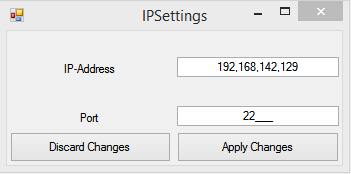
\includegraphics[width=0.7\textwidth]{IP_SETTINGS}\\
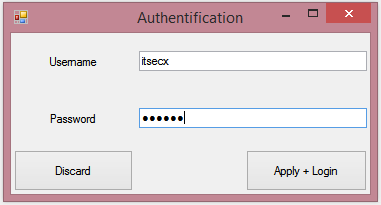
\includegraphics[width=0.7\textwidth]{VERBINDEN}\\
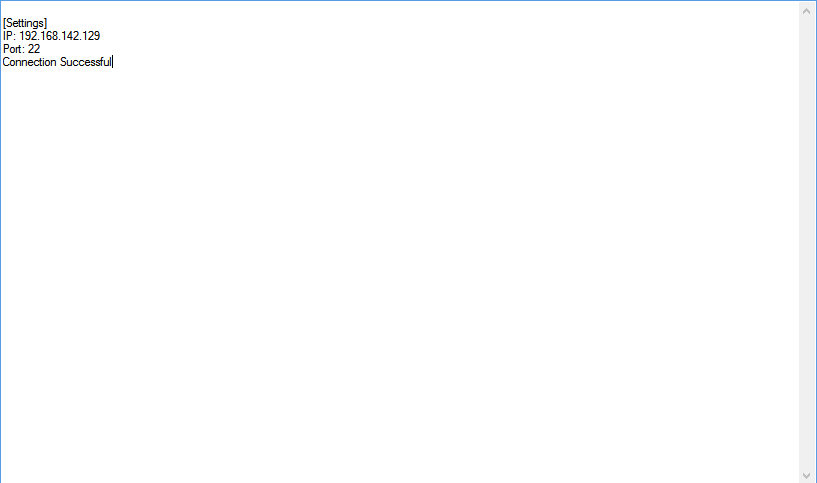
\includegraphics[width=0.7\textwidth]{afterlogin}\\
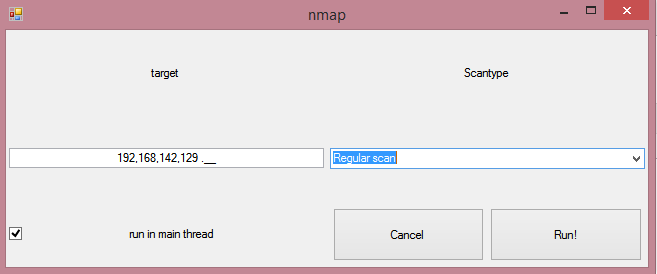
\includegraphics[width=0.7\textwidth]{bsp_nmap}\\
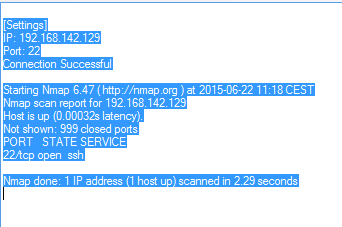
\includegraphics[width=0.7\textwidth]{afternmap}\\
\end{center}
\pagebreak
\section{Rechtliche Hinweise}

\subsection{Haftungsausschluss}
Die Dokumente der ITSecX enthalten Links zu externen Webseiten. 
Die inhalte der externen Webseiten sind implementierungen und nicht
im Angebot inkludiert. 
Die Links sind ausschließlich Verweise zu ergänzenden Information
zu verstehen. 
Auf die Inhalte der verlinkten Webseiten haben wir keinen direkten
Einfluss. 
Zum Zeitpunkt der Verlinkung waren rechtswidrige 
Inhalte nicht erkennbar. 
Falls solche Inhalte zu einem späteren Zeitpunkt bekannt werden sollten,
werden die betreffenden Inhalte angepasst.

\subsection{Lizenz}
Die ITSecX möchte sich Ihnen mit einem erfolgreichem Produkt 
präsentieren. 
Das darin enthaltene geistige Eigentum wie Patente, 
Marken und Urheberrechte ist geschützt.
Durch dieses Produkt wird keine Lizenz zur Nutzung des 
geistigen Eigentums der Marke ITSecX erteilt.

\subsection{Urheberrechte}


© Copyright TGM, 1200 Wien. Alle Rechte vorbehalten. 
Text, Bilder, Grafiken, Sound, Animationen und Videos sowie deren 
Anordnung auf dem ITSecX-Produkt unterliegen dem Schutz des Urheberrechts 
und anderer Schutzgesetze.
\\
Es wird untersagt, den Inhalt dieses Produktes oder Teile davon, 
zu kommerziellen oder auch zu privaten Zwecken zu kopieren, 
zu verbreiten, zu verändern, auf anderen Websites zu verwenden 
oder Dritten zugänglich zu machen.


\end{document}
